\section{Reference Channel Additional Material}
\label{sec:App_RefCh}




\subsection{Plots of fits from systematic study}
\label{subsec:RefCh_fits}

This section contains plots of fits from the systematic studies of the reference channel. Each plot has the systematic being studied and the yield embedded in the upper right. The fit procedure can be found in \ref{subsec:refFit_procedure} and a detailed description of each systematic is found in Section \ref{subsec:refFit_systematics}.


\begin{figure}[h]
    \centering
    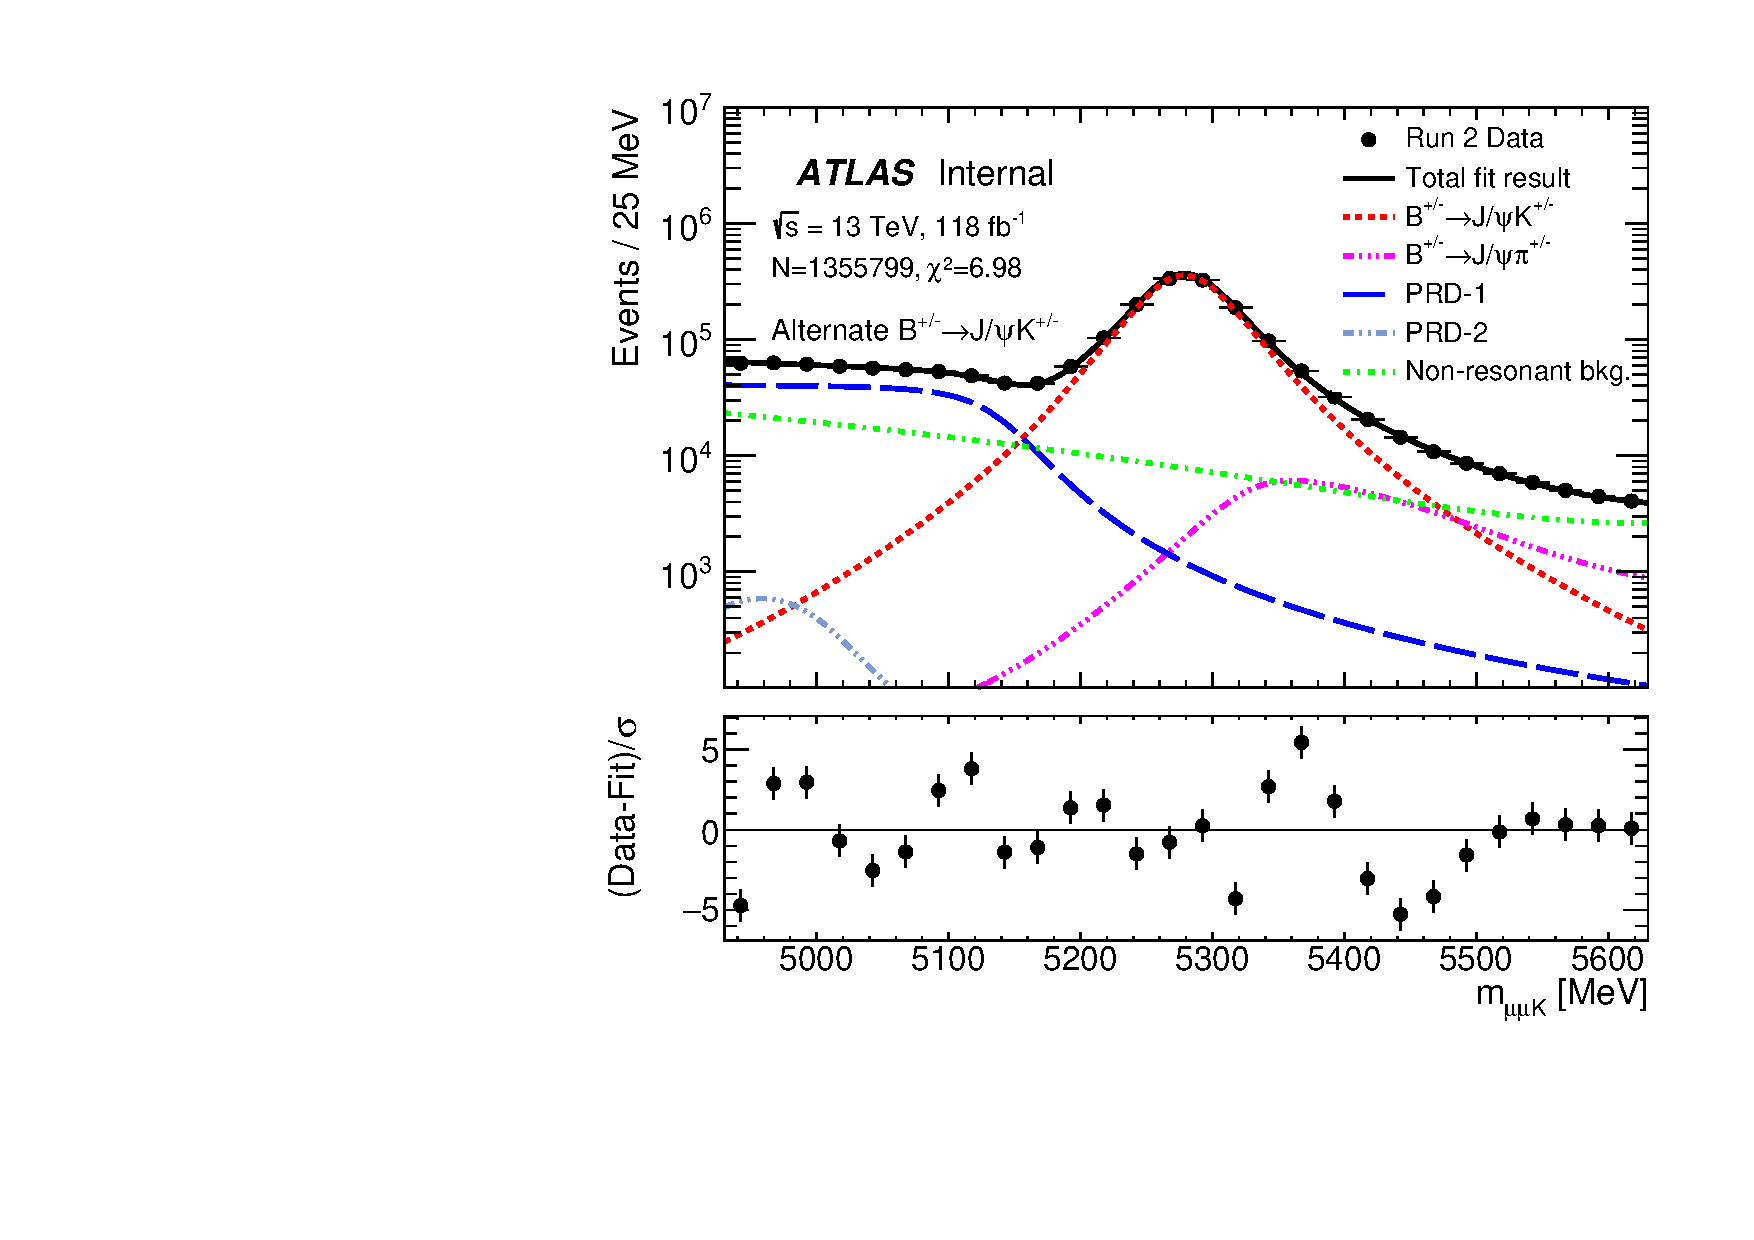
\includegraphics[width=0.6\textwidth]{figures/ReferenceChannel/250519-YieldFit-pdf-1-dataset-0-plot-log}
    \caption{The reference channel fit using a JohnsonSu + Gaussian for the $B^{\pm}\to J\psi K^\pm$ PDF. }
    \label{fig:RefCh-sys-AltBK}
\end{figure}

\begin{figure}[h]
    \centering
    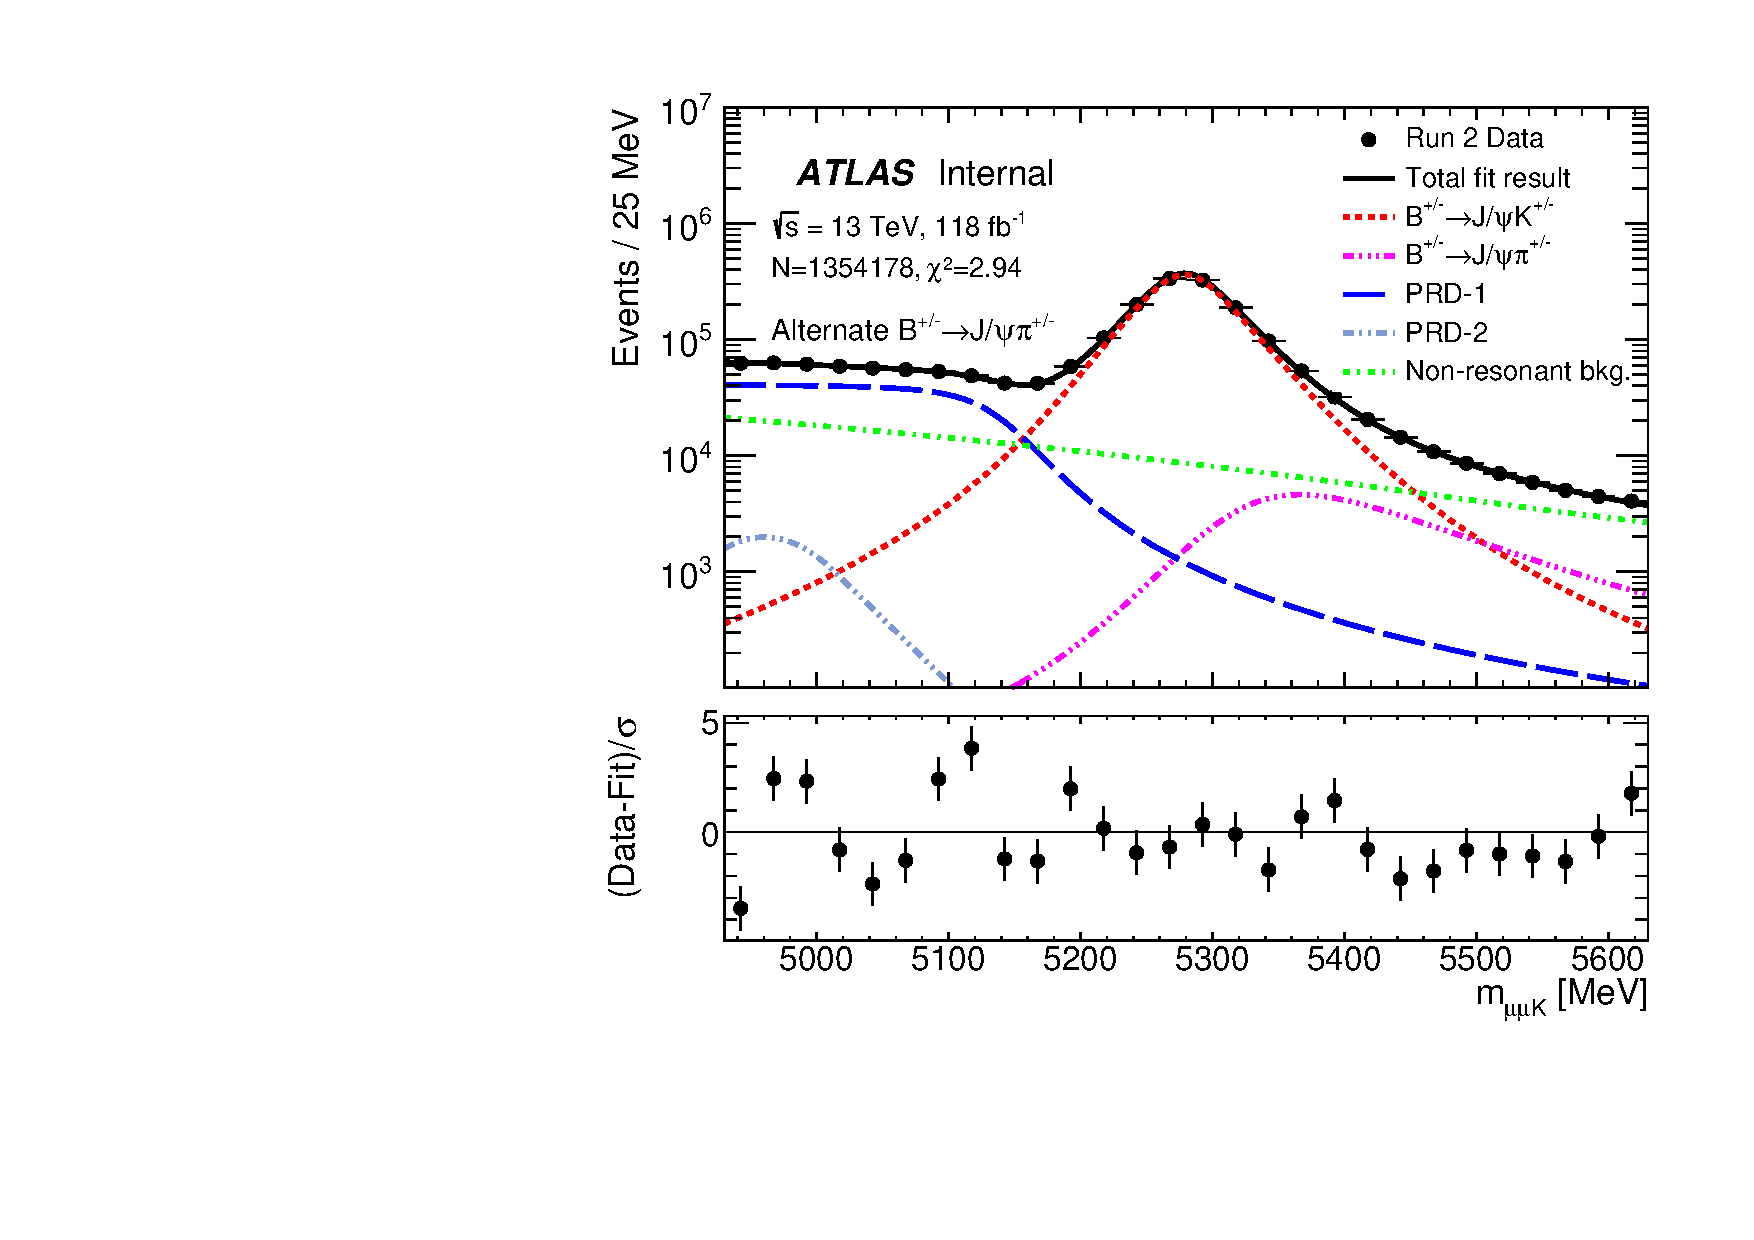
\includegraphics[width=0.6\textwidth]{figures/ReferenceChannel/250519-YieldFit-pdf-2-dataset-0-plot-log}
    \caption{The reference channel fit using a JohnsonSu + JohnsonSu for the $B^{\pm}\to J\psi \pi^\pm$ PDF. }
    \label{fig:RefCh-sys-AltBPi}
\end{figure}

\begin{figure}[h]
    \centering
    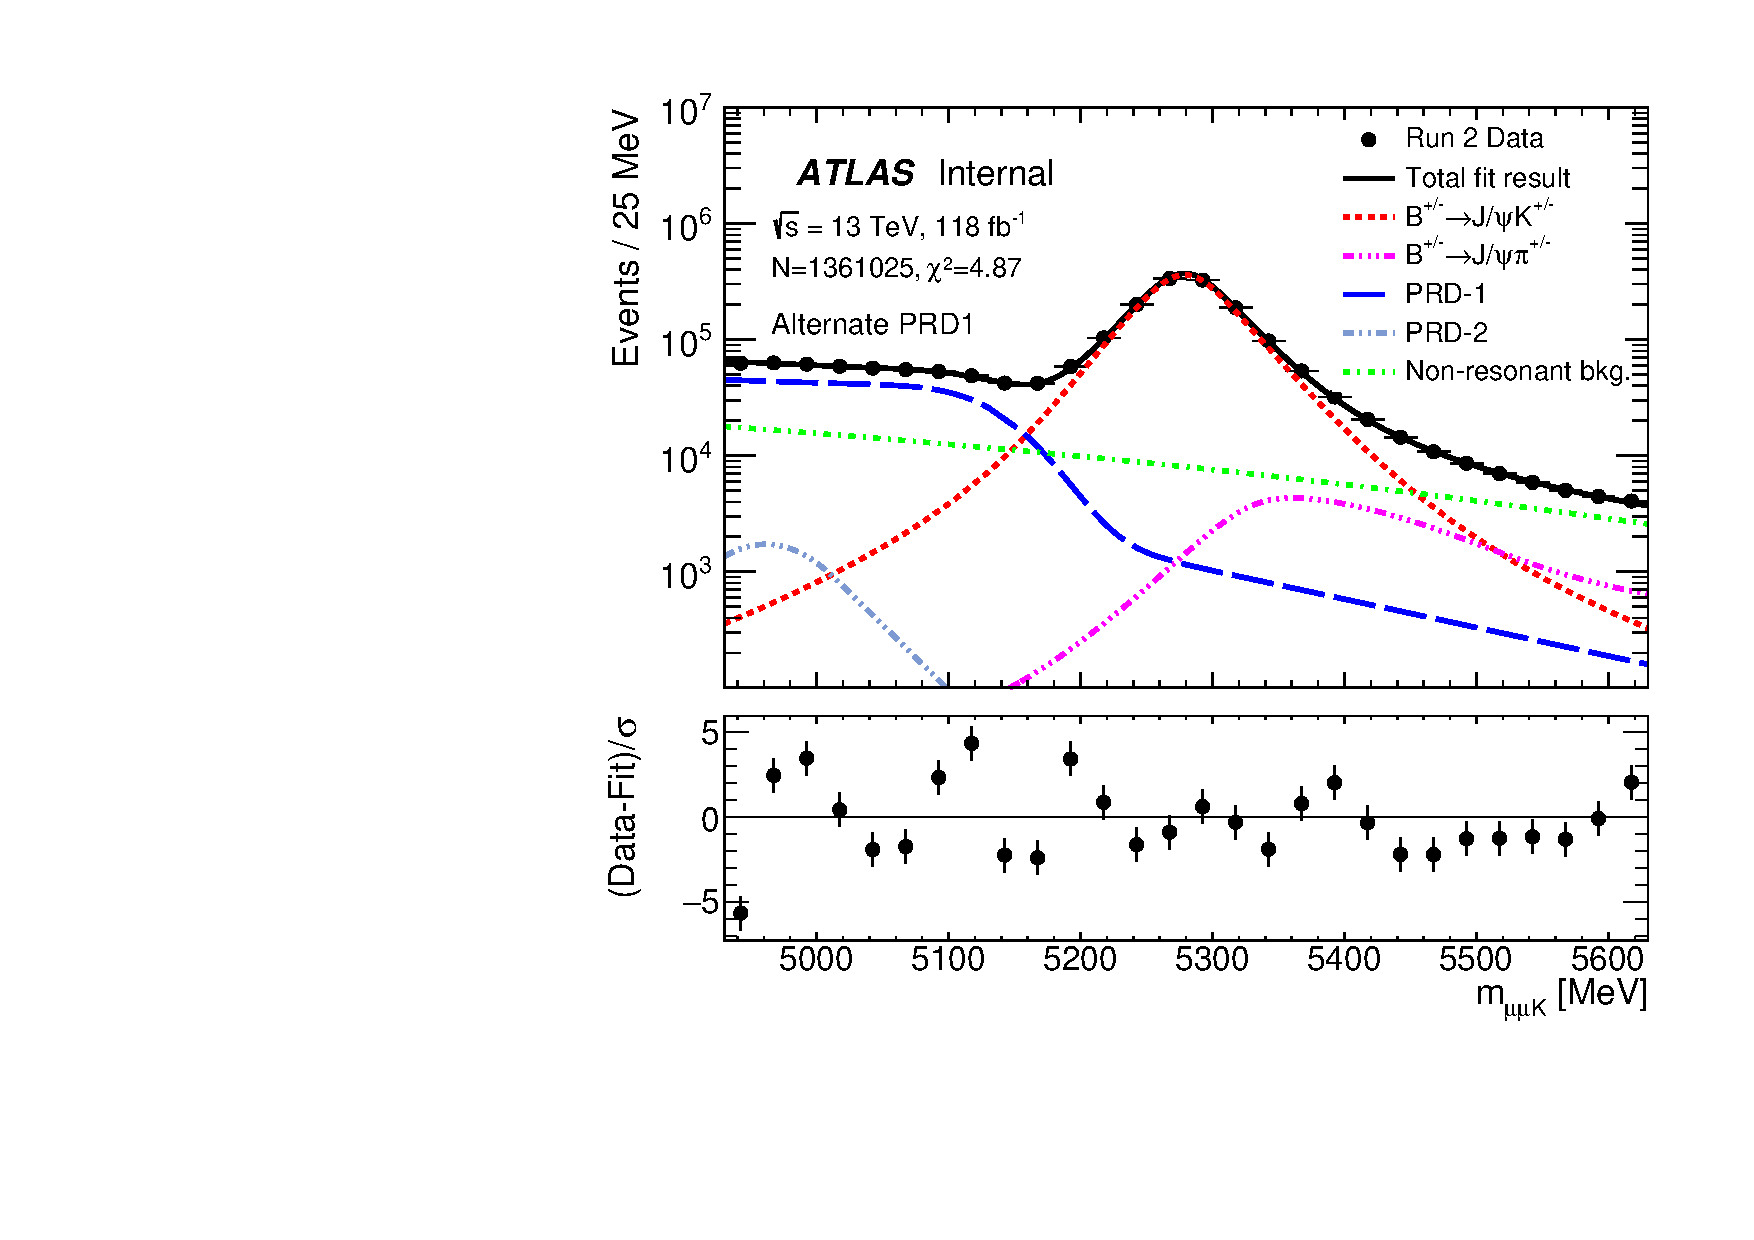
\includegraphics[width=0.6\textwidth]{figures/ReferenceChannel/250522-YieldFit-pdf-3-dataset-0-plot-log}
    \caption{The reference channel fit using a Fermi Dirac + Exponential for the PRD1 PDF. }
    \label{fig:RefCh-sys-AltPRD1}
\end{figure}


\begin{figure}[h]
    \centering
    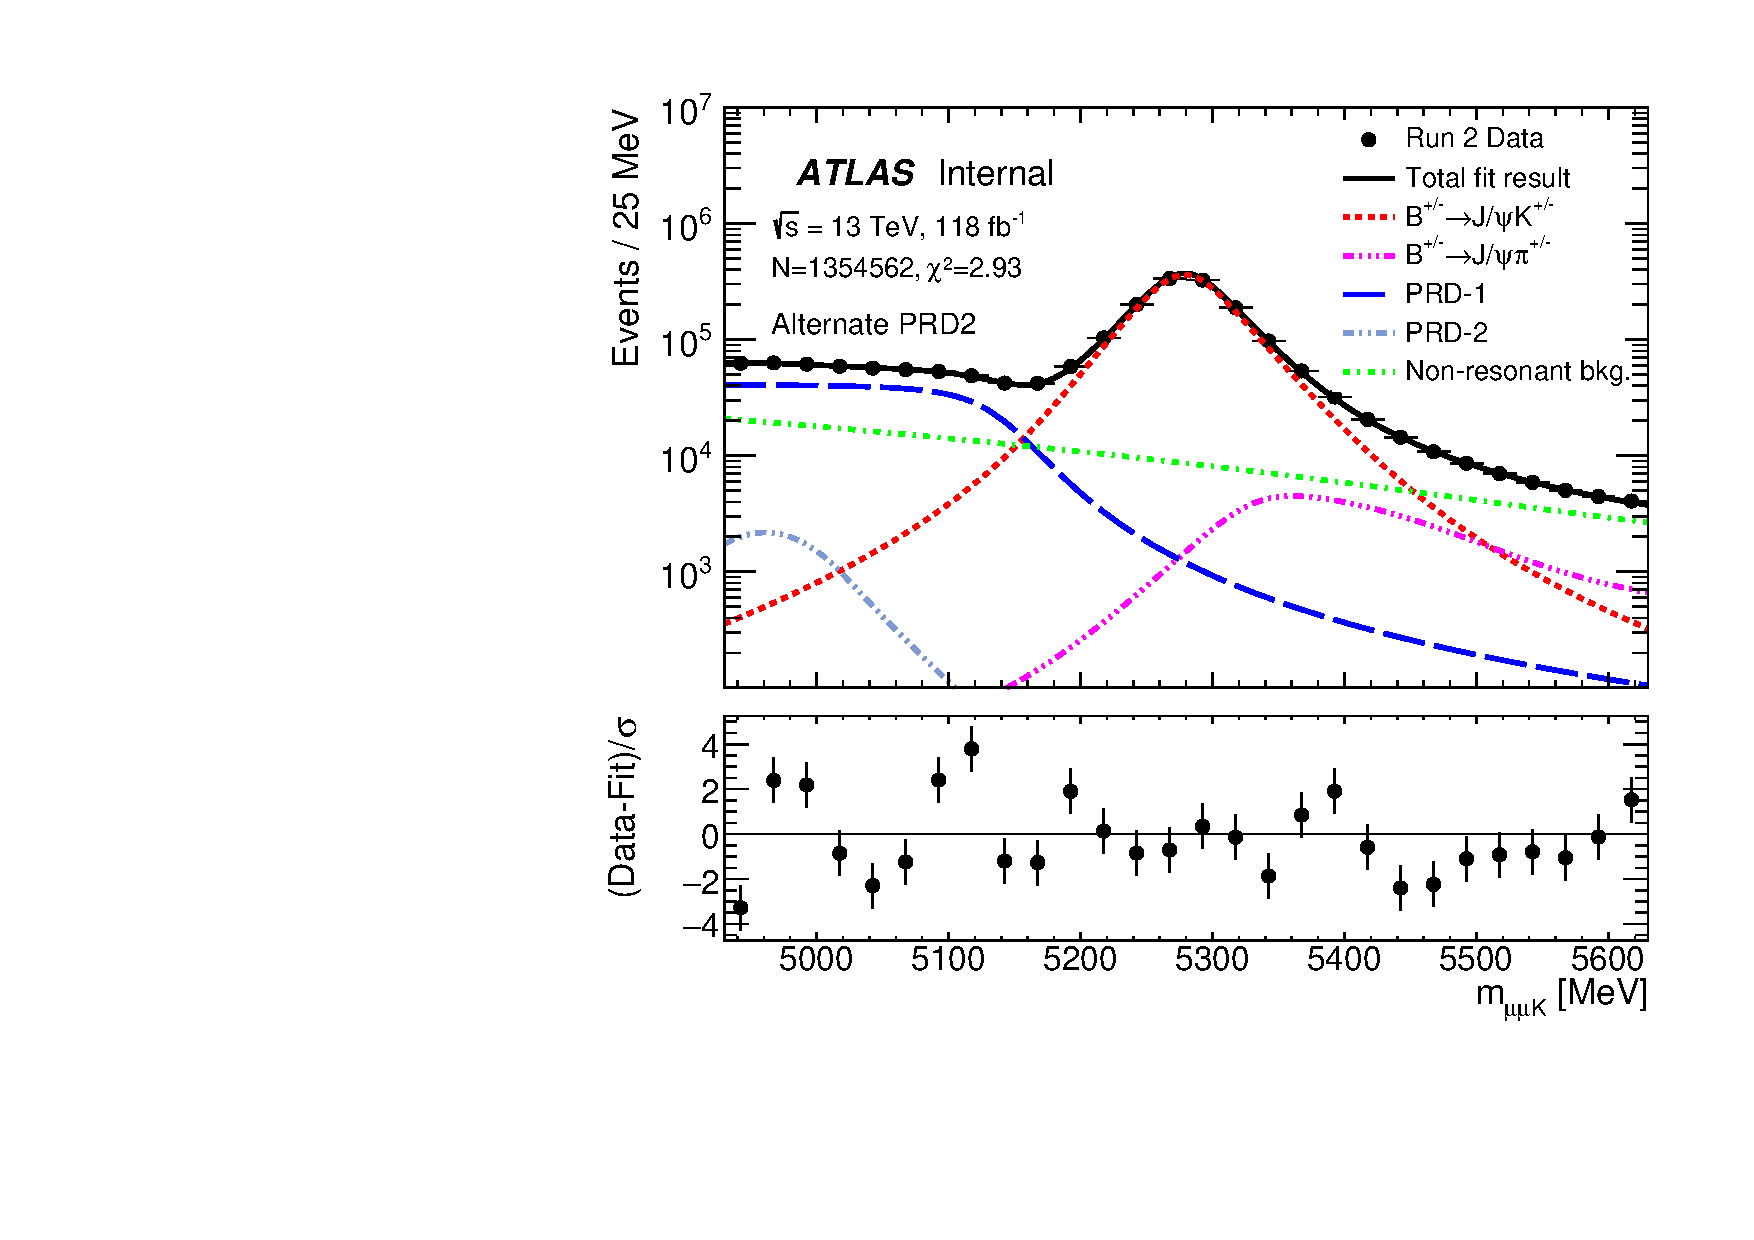
\includegraphics[width=0.6\textwidth]{figures/ReferenceChannel/250519-YieldFit-pdf-4-dataset-0-plot-log}
    \caption{The reference channel fit using a Crystal ball funciton for the PRD2 PDF. }
    \label{fig:RefCh-sys-AltPRD2}
\end{figure}

\begin{figure}[h]
    \centering
    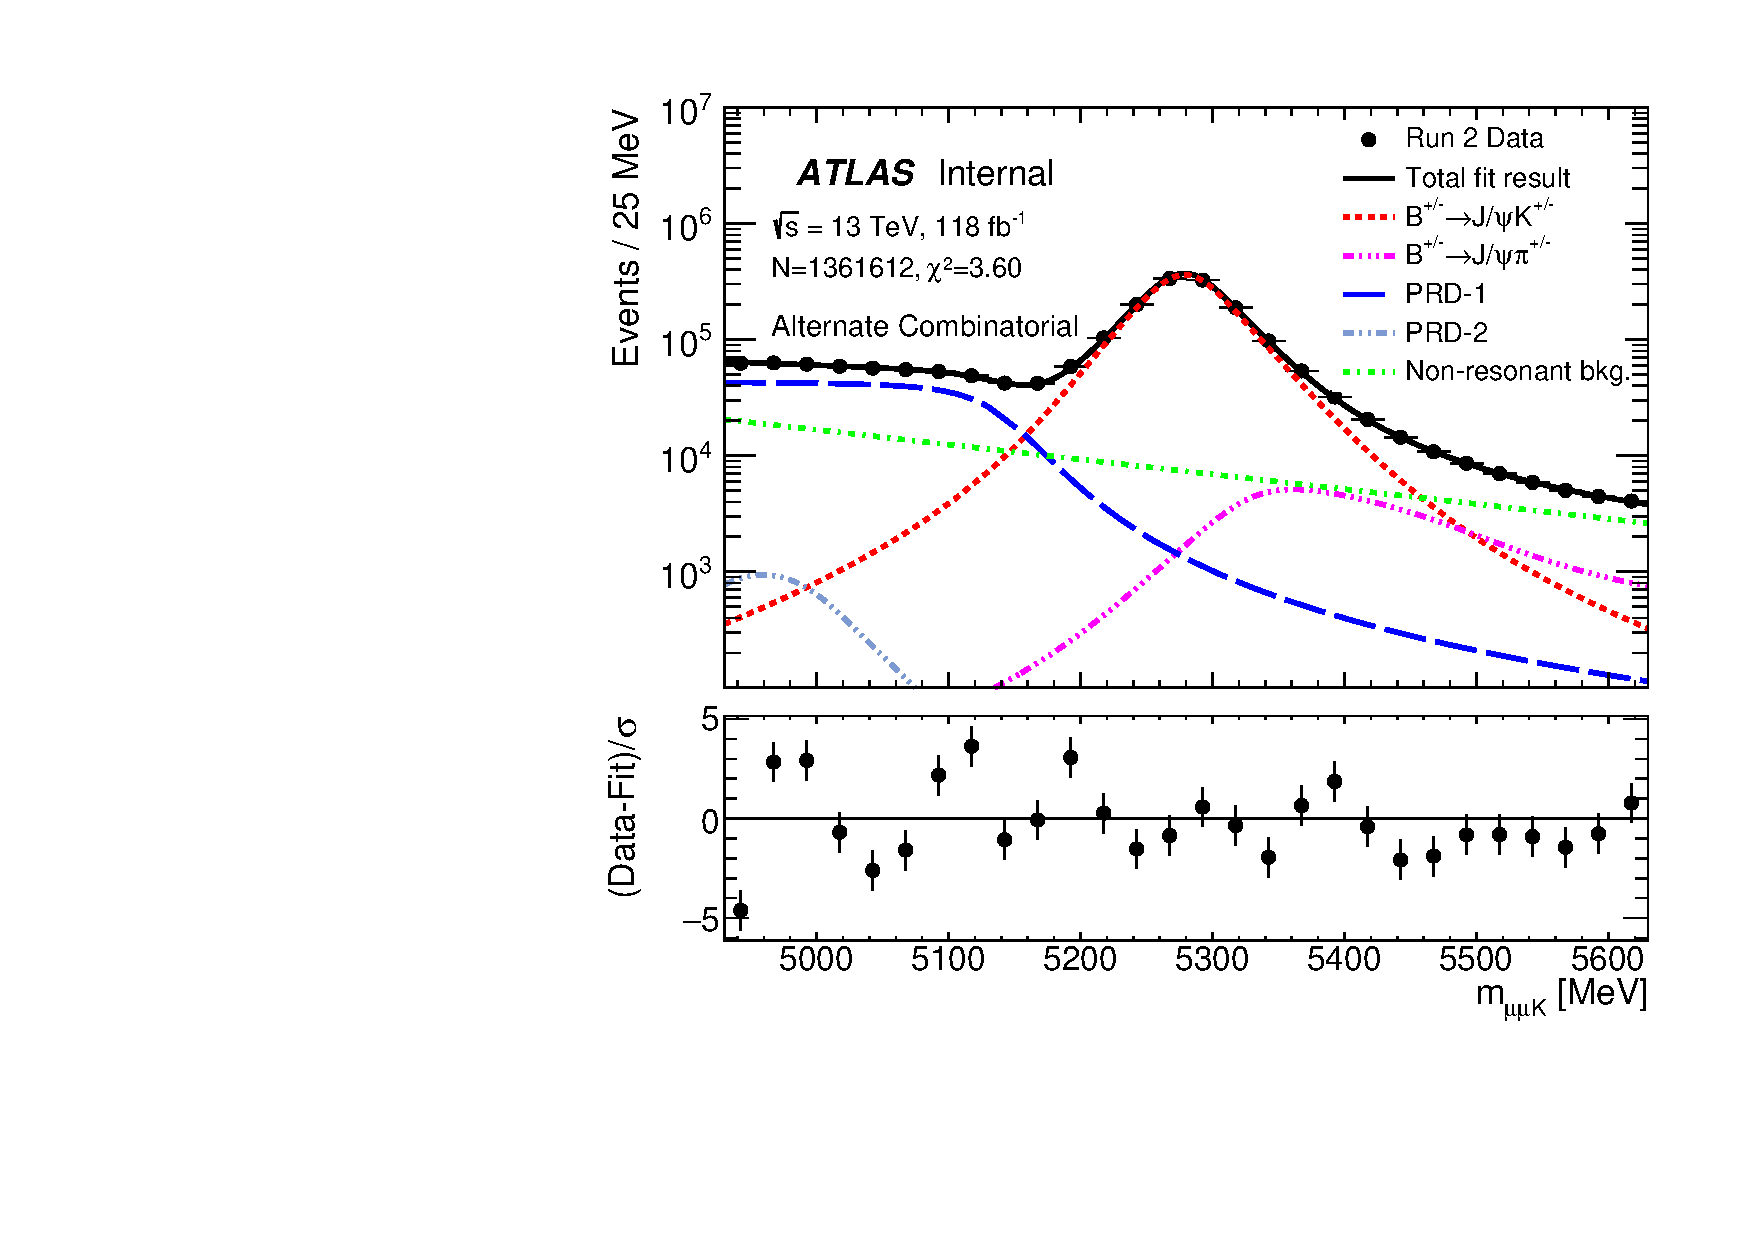
\includegraphics[width=0.6\textwidth]{figures/ReferenceChannel/250522-YieldFit-pdf-5-dataset-0-plot-log}
    \caption{The reference channel fit using a Crystal ball funciton for the Combinatorial PDF. }
    \label{fig:RefCh-sys-AltComb}
\end{figure}